\documentclass[11pt,a4paper, uplatex]{jsarticle}
%
\usepackage{amsmath,amssymb}
\usepackage{bm}
\usepackage[dvipdfmx]{graphicx}
\usepackage{ascmac}
\usepackage{listings,jlisting}
\usepackage{underscore}
\usepackage{subfig}
\lstset{
    frame=single,
    numbers=left,
    tabsize=2
}
%
\setlength{\textwidth}{\fullwidth}
\setlength{\textheight}{40\baselineskip}
\addtolength{\textheight}{\topskip}
\setlength{\voffset}{-0.2in}
\setlength{\topmargin}{0pt}
\setlength{\headheight}{0pt}
\setlength{\headsep}{0pt}
%
\newcommand{\divergence}{\mathrm{div}\,}  %ダイバージェンス
\newcommand{\grad}{\mathrm{grad}\,}  %グラディエント
\newcommand{\rot}{\mathrm{rot}\,}  %ローテーション
%
\title{メディア情報学実験・音声認識 第二週課題レポート}
\author{1510151  栁 裕太}
\date{\today}
\begin{document}

\maketitle
\section{プログラム穴埋め}

\subsection{forward.c}

\begin{lstlisting}[language=c, caption=\texttt{forward}関数一部]
/*------------------------------------
 初期化
------------------------------------*/
t = 0;
for(i=0; i<N; i++) {
  alpha[t][i] = pi[i] * b[i][O[t]];
  /* ここを穴埋めした */;
}

/*------------------------------------
 再帰計算
------------------------------------*/
for(t=0; t<T-1; t++) {
  for(j=0; j<N; j++) {
    sum = 0;
    for(i=0; i<N; i++) {
sum += alpha[t][i] * a[i][j];
      /* ここを穴埋めした */;
    }
    alpha[t+1][j] = sum * b[j][O[t+1]];
    /* ここを穴埋めした */;
  }
}

/*------------------------------------
  forward確率の計算
------------------------------------*/
prob = 0.0;
for(i=0; i<N; i++) {
  prob += alpha[t][i];
  /* ここを穴埋めした */;
}
\end{lstlisting}

\subsection{backward.c}

\begin{lstlisting}[language=c, breaklines = true, caption=\texttt{backward}関数一部]
  /*------------------------------------
    初期化
  ------------------------------------*/
  t = T-1;
  for(i=0; i<=N-1; i++) {
    beta[t][i] = 1
    /* ここを穴埋めした */;
  }

  /*------------------------------------
    再帰計算
  ------------------------------------*/
  for(t=T-2; t>=0; t--) {
    for(i=0; i<N; i++) {
      beta[t][i] = 0;
      for(j=0; j<N; j++) {
	beta[t][i] += a[i][j] * b[j][O[t+1]] * beta[t+1][j];
        /* ここを穴埋めした */;
      }
    }
  }

  /*------------------------------------
    backward確率の計算
  ------------------------------------*/
  prob = 0.0;
  for(i=0; i<N; i++) {
    prob += pi[i] * b[i][O[1]] * beta[1][i];
    /* ここを穴埋めした */;
  }
*/\end{lstlisting}

\subsection{baumwelch.c}

\begin{lstlisting}[language=c, breaklines = true, caption=\texttt{baumWelch}関数一部]
      /*------------------------------------
        πi を再推定
      ------------------------------------*/
      for(i=0; i<N; i++)
        pi[i] = (alpha[1][i] * beta[1][i]) / prob_old;
        /*ここを穴埋め(Algorithm 1の第17行)*/;


      /*------------------------------------
        A (a_ij) を再推定
      ------------------------------------*/
      for(i=0; i<N; i++) {
        for(j=0; j<N; j++) {
    	sum1 = sum2 = 0.0;
          for(t=1; t<=T-1; t++){
            sum1 += alpha[t][i] * a[i][j] * b[j][O[t+1]] * beta[t+1][j];
            sum2 += alpha[t][i] * beta[t][j];
          }
          a[i][j] = sum1 / sum2;
         /*
            ここを穴埋めした
            (Algorithm 1の第21行)*
          */
        }
\end{lstlisting}

\section{各プログラム実行結果}
\subsection{forward}

\begin{lstlisting}[language=c, caption=\texttt{forward}実行結果]
  [~/asr/drill]\% ./forward
  0.0000000	0.0000000	0.0182400	0.0634368
  0.0000000	0.0320000	0.0825600	0.0588096
  0.0000000	0.3840000	0.1459200	0.0120192
  0.8000000	0.0480000	0.0028800	0.0006912
  P(O|λ)= 0.1349568
\end{lstlisting}

\subsection{backward}

\begin{lstlisting}[language=c, caption=\texttt{backward}実行結果]
  [~/asr/drill]\% ./backward
  0.0630000	0.2100000	0.7000000	1.0000000
  0.0713880	0.2274000	0.6700000	1.0000000
  0.1474600	0.2990000	0.4500000	1.0000000
  0.1686960	0.2680000	0.4200000	1.0000000
  P(O|λ)= 0.0536000
\end{lstlisting}

\subsection{baumwelch.c}

\begin{lstlisting}[language=c, breaklines = true, caption=\texttt{baumwelch}実行結果]
  [~/asr/drill]\% baumwelch < d1.txt
  Before Training ---------------
  pi= 1.000000 0.000000
  A=
  0.500000 0.500000
  0.500000 0.500000
  B=
  0.500000 0.500000
  0.500000 0.500000

  Baum-Welch estimation converged.
  After Training ----------------
  pi= 1.000000 0.000000
  A=
  0.256001 0.752594
  0.769426 0.251694
  B=
  0.805410 0.194590
  0.232469 0.767531


  [~/asr/drill]\% baumwelch < d2.txt
  Before Training ---------------
  pi= 1.000000 0.000000
  A=
  0.500000 0.500000
  0.500000 0.500000
  B=
  0.500000 0.500000
  0.500000 0.500000

  Baum-Welch estimation converged.
  After Training ----------------
  pi= 1.000000 0.000000
  A=
  0.730665 0.278419
  0.274128 0.734279
  B=
  0.828889 0.171111
  0.200598 0.799402
\end{lstlisting}

\subsection{recogd}

\begin{lstlisting}[language=c, breaklines = true, caption=\texttt{recogd}実行結果]
  [~/asr/drill]\% recogd data1.list > data1.result
  n1= 93
  n2= 7
  [~/asr/drill]\% recogd data2.list > data2.result
  n1= 7
  n2= 93
\end{lstlisting}

また、recogdの実行結果をグラフ化させたのは以下の図\ref{fig:ps}の通り。

\begin{figure}[h]
  \begin{center}
    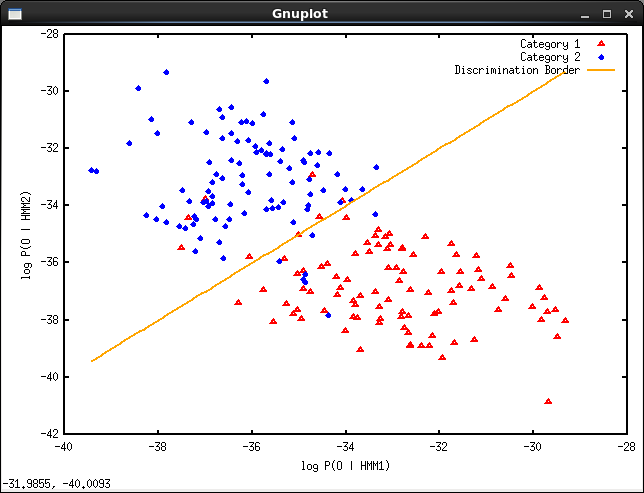
\includegraphics[width=13.0cm]{recog-l2-result.png}
    \caption{実行結果グラフ}
    \label{fig:ps}
  \end{center}
\end{figure}


\section{実験のポイント}

今回の実験では、隠れマルコフモデル(HMM)の$P(O|λ)$の効率的な算法であるForwardアルゴリズムと
Backwardアルゴリズムを、手元の手計算とC言語アルゴリズム化の2方向から体験した。
また、それを元に実際にパラメータ推定(Baum-Welch)アルゴリズムのC言語上での実装を行うことで、
実際にHMMによる認識実験を行った。

最大のポイントは、Forward・Backwardアルゴリズムの内容を深く理解する点にあると考えている。
これは、効率的な$P(O|λ)$の導出方法を知ることで、演算回数を大幅に減らすことで、
一気に機械認識のハードルを下げることにつながるためである。

\section{よくわかったこと}

Forward・Backwardアルゴリズムの挙動を、手計算・C言語実装で深く理解することができた。

\section{よくわからなかったこと}

Forward・Backwardアルゴリズムによって$P(O|λ)$の導出への負担を大幅に減らすことができる…
らしいが、実際どれぐらい処理速度が速くなるのか知ることができなかった。

\section{要望}

baumwelch・recogdプログラム実装には、想定より多くの落とし穴があった
(値変更忘れ、for文の繰り返し変数上限・下限の設定など)。
この影響でミスに気付くのに時間がとられ、作業効率が落ちてしまった。
これらに関してはTAチェックの際に、チェックリストのようなものがあると、迅速にミスに気付ける可能性がある。

\section{感想・その他}

来週、HMMを活用した音声認識を行うということで、どのようなものになるか楽しみである。

\end{document}
